\documentclass[11pt]{article}

\usepackage[margin=1in]{geometry}
\usepackage{amsmath, amssymb, amsthm}
\usepackage{array}
\usepackage{booktabs}
\usepackage{enumitem}
\usepackage{graphicx}
\usepackage{hyperref}
\usepackage{pgfplots}
\usepackage[most]{tcolorbox}
\usepackage[table]{xcolor}
\usepackage{tikz}
\usetikzlibrary{arrows.meta,fit,positioning}
\pgfplotsset{compat=1.18}

\newcolumntype{L}[1]{>{\raggedright\arraybackslash}p{#1}}
\newcommand{\calendarentry}[1]{\rule{0pt}{2.9ex}#1}
\definecolor{SoftBlue}{HTML}{EEF6FC}
\definecolor{FrameBlue}{HTML}{2C6E91}
\definecolor{SoftGold}{HTML}{FFF4E5}
\definecolor{FrameGold}{HTML}{A55F00}
\definecolor{SoftGreen}{HTML}{EAF7ED}
\definecolor{FrameGreen}{HTML}{2E7D32}

\setlength{\parindent}{0pt}
\setlength{\parskip}{0.45em}
\setlist[itemize]{leftmargin=1.6em,labelsep=0.55em,itemsep=0.2em,topsep=0.3em,parsep=0pt,partopsep=0pt}
\setlist[enumerate]{leftmargin=1.8em,labelsep=0.5em,itemsep=0.2em,topsep=0.3em,parsep=0pt,partopsep=0pt}

\newtcolorbox{examplebox}[1][]{
    enhanced,
    breakable,
    colback=SoftBlue,
    colframe=FrameBlue,
    boxrule=0.9pt,
    arc=2pt,
    left=8pt,
    right=8pt,
    top=6pt,
    bottom=6pt,
    fonttitle=\bfseries,
    #1
}

\newtcolorbox{keybox}[1][]{
    enhanced,
    breakable,
    colback=SoftGold,
    colframe=FrameGold,
    boxrule=0.9pt,
    arc=2pt,
    left=8pt,
    right=8pt,
    top=6pt,
    bottom=6pt,
    fonttitle=\bfseries,
    #1
}

\newtcolorbox{reviewbox}[1][]{
    enhanced,
    breakable,
    colback=SoftGreen,
    colframe=FrameGreen,
    boxrule=0.9pt,
    arc=2pt,
    left=8pt,
    right=8pt,
    top=6pt,
    bottom=6pt,
    fonttitle=\bfseries,
    #1
}

\title{First Two-Class Appointment Simulation: Day-Level Formulation v2}
\author{Alexandre SEPULVEDA de DIETRICH\\Under the supervision of Pr.~Carri Chan}
\date{\today}

\begin{document}
\maketitle
\setcounter{tocdepth}{3}
\tableofcontents
\bigskip

\section{Introduction}

\subsection{Purpose and Reader Map}

This v2 note is the day-level replacement for the earlier slot-level formulation. The earlier
note remains useful because it showed the model through concrete pictures: a time-evolution graph,
a rolling calendar table, a cancellation-hazard plot, and a worked FCFS appointment book. This
version keeps that teaching style, but changes the model state to day/class counts.

\begin{keybox}[title={Core Modeling Choice}]
The simulation clock is the day \(D\). The model state records how many patients of each class are
scheduled on each residual day. The code may keep internal slot positions to enforce capacity and
audit utilization, but slot position \(m\) is no longer a model state variable.
\end{keybox}

\subsubsection{What Changed from the Previous Note}

The table below records what the old note used to help a reader understand the simulator and the
equivalent object in the day-level formulation.

\begin{center}
\small
\begin{tabular}{L{0.28\textwidth} L{0.28\textwidth} L{0.34\textwidth}}
\toprule
\textbf{Old explanatory device} & \textbf{What it taught} & \textbf{Day-level v2 replacement} \\
\midrule
Slot epoch \(t=(D,s)\) and rollover graph & how the simulator moved through slots inside a day & daily epoch graph \(D\to D+1\) with the seven explicit daily events \\
\addlinespace
Slot calendar \(Y_t(r,m)\) & where each booked appointment sat in the rolling calendar & class-count state \(X_{i,r}^{D}\) plus aggregate occupancy \(N_r^D\) by residual day \\
\addlinespace
Colored \(H\times S\) appointment book & how FCFS filled slots and how holes appeared & colored residual-day table showing total load, open capacity, and future-only offers \\
\addlinespace
No-show and cancellation plots & how baseline step rules differ from the smoother legacy delay-sensitive functions & baseline \(\xi_i(\tau)\) and \(\phi_i\) in solid lines, with advanced \(\tilde{\xi}_i(\tau)\) and \(\tilde{\phi}_i(\tau,r)\) shown as dashed later options \\
\addlinespace
Worked FCFS example & how a request becomes an offer, booking, balk, no-show, or service & day-level progression example with cancellations, arrivals, offers, balking, service, metrics, and calendar advance \\
\addlinespace
Metric tables & how logs map to access and utilization measures & same metrics, plus the \texttt{daily\_progression} audit table that records every daily step \\
\bottomrule
\end{tabular}
\normalsize
\end{center}

\section{Model Formulation}

\subsection{Model at a Glance}

The simulator keeps the same operational feedback loop as the earlier model and the motivating
appointment-queueing literature.

\begin{keybox}[title={Core Feedback Loop}]
\begin{align*}
\text{more backlog}
&\Rightarrow
\text{larger offered delay}\\
&\Rightarrow
\text{more balking, cancellation, or no-show risk}\\
&\Rightarrow
\text{lower realized service}.
\end{align*}
\end{keybox}

The day-level objects are:
\begin{itemize}[nosep]
    \item \(D\): current calendar day.
    \item \(S\): number of appointment slots available per day.
    \item \(H\): rolling booking horizon in days.
    \item \(\mathcal I\): set of patient classes, equal to \(\{1,2\}\) in the first experiments.
    \item \(r\in\{0,1,\dots,H-1\}\): residual delay, where \(r=0\) means appointments scheduled for today.
    \item \(\tau\): original offered delay accepted by a booked patient.
\end{itemize}

The main distinction remains:
\begin{keybox}[title={Residual Delay vs. Original Delay}]
Residual delay \(r\) belongs to the day-level state and decreases as days pass. Original delay
\(\tau\) is stored with the booked patient because balking, optional advanced cancellation rules, and
no-show behavior may depend on the delay the patient accepted.
\end{keybox}

\subsection{Day-Level State}

At the start of day \(D\), after the future-day cancellation step and before processing new arrivals,
define
\[
X_{i,r}^{D}
=
\text{number of class-}i\text{ patients scheduled for day }D+r.
\]

The state vector is
\[
X^D=\left(X_{i,r}^{D}:i\in\mathcal I,\ r=0,\dots,H-1\right).
\]

For each residual day, aggregate occupancy is
\[
N_r^D=\sum_{i\in\mathcal I}X_{i,r}^{D},
\]
and daily capacity imposes
\[
N_r^D\le S.
\]

Slot positions inside a day are not part of \(X^D\). The implementation still keeps an internal
list of \(S\) slots per day so it can find open capacity, produce service-slot logs, and compute
empty-slot utilization. That internal detail is an audit layer, not the mathematical state.

\subsubsection{Patient Audit Record}

When a class-\(i\) patient accepts an offer with delay \(\tau\), the state count is incremented on
the selected residual day, and the implementation also stores a patient audit record
\[
(i,\tau).
\]

The audit record is needed because:
\begin{itemize}[nosep]
    \item \(b_i(\tau)\) determines balking when the offer is made;
    \item baseline \(\xi_i(\tau)\) determines no-show at appointment time;
    \item advanced no-show experiments may instead use \(\tilde{\xi}_i(\tau)\);
    \item optional advanced cancellation functions may use \(\tilde{\phi}_i(\tau,r)\);
    \item cohort logs and delay metrics need the originally offered delay.
\end{itemize}

\subsection{Patient Classes and Behavior}

Each class is described by
\[
C_i=\{\lambda_i,b_i(\tau),\phi_i,\xi_i(\tau)\}.
\]

\begin{center}
\small
\begin{tabular}{L{0.22\textwidth} L{0.68\textwidth}}
\toprule
\textbf{Object} & \textbf{Meaning} \\
\midrule
\(\lambda_i\) & expected number of class-\(i\) arrivals per day \\
\addlinespace
\(b_i(\tau)\) & probability that class-\(i\) declines an offered appointment with delay \(\tau\) \\
\addlinespace
\(\phi_i\) & scalar daily cancellation probability for class-\(i\) patients scheduled on future days \\
\addlinespace
\(\tilde{\phi}_i(\tau,r)\) & advanced daily cancellation rule using original delay and residual delay; not used in the baseline FCFS analysis \\
\addlinespace
\(\xi_i(\tau)\) & baseline step no-show probability at appointment time if the patient has not canceled \\
\addlinespace
\(\tilde{\xi}_i(\tau)\) & advanced delay-sensitive no-show rule; not used in the baseline FCFS analysis \\
\bottomrule
\end{tabular}
\normalsize
\end{center}

The baseline cancellation input is \(\phi_i\). It is applied directly once per day to every
class-\(i\) patient still scheduled on a future day \(D+r\), \(r\in\{1,\dots,H-1\}\), when the daily
cancellation step is executed. It is not converted from an eventual cancellation probability.

For two-class experiments, demand can also be parameterized by total daily arrival volume
\(\lambda\) and class-1 share \(p\):
\[
\lambda_1=p\lambda,\qquad
\lambda_2=(1-p)\lambda.
\]

\subsubsection{Working Behavior Profile}

The first FCFS experiments use a concrete two-class profile. The numbers below are not required by
the model, but they make the figures and examples reproducible.

\begin{center}
\small
\begin{tabular}{L{0.24\textwidth} L{0.31\textwidth} L{0.31\textwidth}}
\toprule
\textbf{Object} & \textbf{Class 1: MRI-like diagnostic} & \textbf{Class 2: behavioral-health follow-up} \\
\midrule
Daily demand & \(\lambda_1=14\) when \(\lambda=24\) and \(p=7/12\) & \(\lambda_2=10\) when \(\lambda=24\) and \(p=7/12\) \\
\addlinespace
Balking & low until a 21-day access threshold, then high & low until a 14-day access threshold, then high \\
\addlinespace
No-show & step \(\xi_1(\tau)\): 0.01 before 21 days, 0.31 from 21 days onward; dashed \(\tilde{\xi}_1(\tau)\) reserved for later & step \(\xi_2(\tau)\): 0.15 before 14 days, 0.51 from 14 days onward; dashed \(\tilde{\xi}_2(\tau)\) reserved for later \\
\addlinespace
Cancellation & scalar \(\phi_1=0.01\) in the baseline; advanced \(\tilde{\phi}_1(\tau,r)\) is reserved for later experiments & scalar \(\phi_2=0.02\) in the baseline; advanced \(\tilde{\phi}_2(\tau,r)\) is reserved for later experiments \\
\bottomrule
\end{tabular}
\normalsize
\end{center}

\subsubsection{Balking Function}

In the current FCFS baseline, balking is represented with a step function of the offered delay.
This is intentionally simple: patients are fairly willing to accept appointments below a practical
access threshold, and much less willing once the offered delay crosses that threshold.

\[
b_1(\tau)=
\begin{cases}
0.02, & \tau<21,\\
0.55, & \tau\ge 21,
\end{cases}
\qquad
b_2(\tau)=
\begin{cases}
0.04, & \tau<14,\\
0.72, & \tau\ge 14.
\end{cases}
\]

\begin{examplebox}[title={Balking as a Step Function of Delay}, breakable=false]
\begin{center}
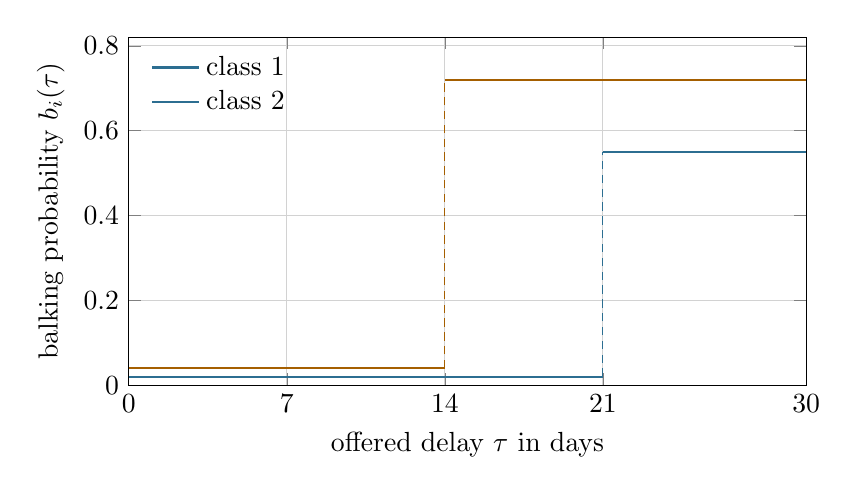
\begin{tikzpicture}
\begin{axis}[
    width=0.84\linewidth,
    height=6.0cm,
    xlabel={offered delay \(\tau\) in days},
    ylabel={balking probability \(b_i(\tau)\)},
    xmin=0,
    xmax=30,
    ymin=0,
    ymax=0.82,
    xtick={0,7,14,21,30},
    ytick={0,0.2,0.4,0.6,0.8},
    scaled y ticks=false,
    yticklabel style={/pgf/number format/fixed,/pgf/number format/precision=2},
    grid=both,
    grid style={gray!20},
    major grid style={gray!35},
    legend style={draw=none, fill=none, at={(0.02,0.98)}, anchor=north west},
]
\addplot[thick, color=FrameBlue, domain=0:21, samples=2] {0.02};
\addlegendentry{class 1}
\addplot[thick, color=FrameBlue, domain=21:30, samples=2] {0.55};
\addplot[densely dashed, color=FrameBlue] coordinates {(21,0.02) (21,0.55)};

\addplot[thick, color=FrameGold, domain=0:14, samples=2] {0.04};
\addlegendentry{class 2}
\addplot[thick, color=FrameGold, domain=14:30, samples=2] {0.72};
\addplot[densely dashed, color=FrameGold] coordinates {(14,0.04) (14,0.72)};
\end{axis}
\end{tikzpicture}
\end{center}

The operational interpretation is direct. Under FCFS, congestion increases the first available
future residual day. Once that offered delay crosses a class-specific threshold, many more patients
decline the offer. This is the access-side version of the same delay feedback loop that the
literature usually models through no-show behavior.
\end{examplebox}

\subsubsection{No-Show Function}

No-show behavior uses the original accepted delay \(\tau\), not the residual delay \(r\) on a later
day. In the current FCFS baseline, no-show is represented with a step function, just like balking:
\[
\xi_1(\tau)=
\begin{cases}
0.01, & \tau<21,\\
0.31, & \tau\ge 21,
\end{cases}
\qquad
\xi_2(\tau)=
\begin{cases}
0.15, & \tau<14,\\
0.51, & \tau\ge 14.
\end{cases}
\]

The earlier Green-Savin style delay-sensitive curve is still useful as an advanced option for later
experiments. In this note it is written as
\[
\tilde{\xi}_i(\tau)
=
\gamma_{i,\max}
-
(\gamma_{i,\max}-\gamma_{i,0})e^{-\tau/s_i}.
\]
For the same illustrative values,
\[
(\gamma_{1,0},\gamma_{1,\max},s_1)=(0.01,0.31,50),
\qquad
(\gamma_{2,0},\gamma_{2,\max},s_2)=(0.15,0.51,9).
\]

\begin{examplebox}[title={Baseline Step No-Show and Advanced \texorpdfstring{$\tilde{\xi}$}{xi-tilde}}, breakable=false]
\begin{center}
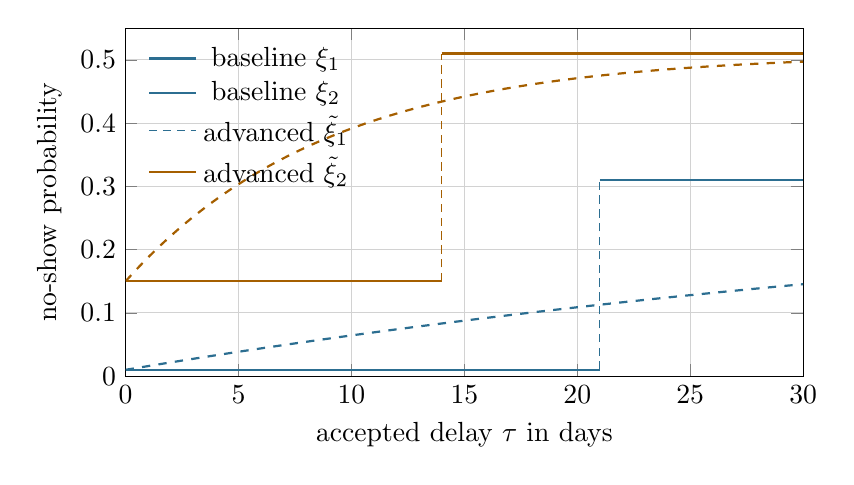
\begin{tikzpicture}
\begin{axis}[
    width=0.84\linewidth,
    height=6.0cm,
    xlabel={accepted delay \(\tau\) in days},
    ylabel={no-show probability},
    xmin=0,
    xmax=30,
    ymin=0,
    ymax=0.55,
    xtick={0,5,10,15,20,25,30},
    ytick={0,0.1,0.2,0.3,0.4,0.5},
    scaled y ticks=false,
    yticklabel style={/pgf/number format/fixed,/pgf/number format/precision=2},
    grid=both,
    grid style={gray!20},
    major grid style={gray!35},
    legend style={draw=none, fill=none, at={(0.02,0.98)}, anchor=north west},
]
\addplot[thick, color=FrameBlue, domain=0:21, samples=2] {0.01};
\addlegendentry{baseline \(\xi_1\)}
\addplot[thick, color=FrameBlue, domain=21:30, samples=2] {0.31};
\addplot[densely dashed, color=FrameBlue] coordinates {(21,0.01) (21,0.31)};

\addplot[thick, color=FrameGold, domain=0:14, samples=2] {0.15};
\addlegendentry{baseline \(\xi_2\)}
\addplot[thick, color=FrameGold, domain=14:30, samples=2] {0.51};
\addplot[densely dashed, color=FrameGold] coordinates {(14,0.15) (14,0.51)};

\addplot[smooth, thick, dashed, color=FrameBlue, domain=0:30, samples=120] {0.31 - (0.31 - 0.01)*exp(-x/50)};
\addlegendentry{advanced \(\tilde{\xi}_1\)}
\addplot[smooth, thick, dashed, color=FrameGold, domain=0:30, samples=120] {0.51 - (0.51 - 0.15)*exp(-x/9)};
\addlegendentry{advanced \(\tilde{\xi}_2\)}
\end{axis}
\end{tikzpicture}
\end{center}

The solid curves are the implemented baseline. They make the daily progression easier to read:
patients who accepted a short delay behave one way, and patients who accepted a longer delay behave
another way. The dashed curves show the smoother advanced \(\tilde{\xi}_i(\tau)\) option, which is
closer to Green-Savin style delay sensitivity and remains available for later experiments.
\end{examplebox}

\begin{examplebox}[title={Cancellation Probability Figure: Baseline and Advanced Rule}]
The new baseline uses a constant daily cancellation probability \(\phi_i\). The older
delay/residual-delay function is renamed
\[
\tilde{\phi}_i(\tau,r),
\]
and is kept only as an advanced option for later experiments. It is not part of the baseline FCFS
analysis in this note.

For example, the advanced taper has the form
\[
\tilde{\phi}_i(\tau,r)
=
\min\{a_i+c_i\tau,\bar{\phi}_i\}\frac{r}{\tau},
\qquad 1\le r\le \tau,
\]
with \(\tilde{\phi}_i(\tau,0)=0\). The figure shows the difference between the scalar baseline and
that advanced option.

\begin{center}
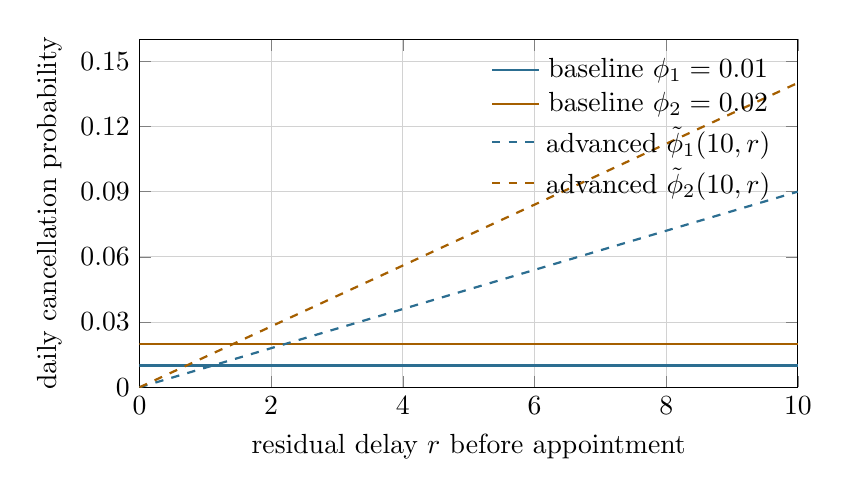
\begin{tikzpicture}
\begin{axis}[
    width=0.82\linewidth,
    height=6.0cm,
    xlabel={residual delay \(r\) before appointment},
    ylabel={daily cancellation probability},
    xmin=0,
    xmax=10,
    ymin=0,
    ymax=0.16,
    xtick={0,2,4,6,8,10},
    ytick={0,0.03,0.06,0.09,0.12,0.15},
    scaled y ticks=false,
    yticklabel style={/pgf/number format/fixed,/pgf/number format/precision=2},
    grid=both,
    grid style={gray!20},
    major grid style={gray!35},
    legend style={draw=none, fill=none, at={(0.98,0.98)}, anchor=north east},
]
\addplot[thick, color=FrameBlue, domain=0:10, samples=2] {0.01};
\addlegendentry{baseline \(\phi_1=0.01\)}
\addplot[thick, color=FrameGold, domain=0:10, samples=2] {0.02};
\addlegendentry{baseline \(\phi_2=0.02\)}
\addplot[thick, dashed, color=FrameBlue, domain=0:10, samples=100] {(0.01+0.008*10)*x/10};
\addlegendentry{advanced \(\tilde{\phi}_1(10,r)\)}
\addplot[thick, dashed, color=FrameGold, domain=0:10, samples=100] {(0.02+0.012*10)*x/10};
\addlegendentry{advanced \(\tilde{\phi}_2(10,r)\)}
\end{axis}
\end{tikzpicture}
\end{center}

The flat lines are the implemented baseline: each scheduled class-\(i\) patient faces the same
daily probability \(\phi_i\) on each day they are considered. The dashed curves are only an example
of the advanced \(\tilde{\phi}_i(\tau,r)\) rule, where risk can vary with both the original delay
and the residual delay.
\end{examplebox}

\section{Simulation Mechanics}

\subsection{Daily Simulation Order}

The simulator advances one day at a time. For each day \(D\), it executes the following steps in
this exact order.

\begin{enumerate}[itemsep=0.35em]
    \item \textbf{Compute cancellations for the day.} Each class-\(i\) patient scheduled for a future day \(D+r\), \(r\in\{1,\dots,H-1\}\), independently cancels with daily probability \(\phi_i\).
    \item \textbf{Simulate daily arrivals.}
    \[
    M_i^D\sim\mathrm{Poisson}(\lambda_i),
    \]
    where \(M_i^D\) is the number of class-\(i\) arrivals on day \(D\).
    \item \textbf{Offer future days in FCFS order.} Arrivals are processed sequentially in randomized within-day order. The baseline policy offers the earliest future day \(D+r\), \(r\in\{1,\dots,H-1\}\), with open capacity.
    \item \textbf{Simulate balking.} A class-\(i\) patient offered delay \(\tau=r\) accepts with probability \(1-b_i(\tau)\). If the patient balks, the capacity remains open for later arrivals.
    \item \textbf{Simulate no-shows and service for day \(D\).} Each remaining appointment scheduled for \(D\) no-shows with baseline probability \(\xi_i(\tau)\), using its stored original delay.
    \item \textbf{Compute metrics for day \(D\).} The simulator records access, booking, cancellation, service, empty-slot, utilization, and delay metrics.
    \item \textbf{Advance to day \(D+1\).} The current day is removed, residual delays decrease by one, and a new empty future day is appended.
\end{enumerate}

\begin{center}
\resizebox{0.98\linewidth}{!}{
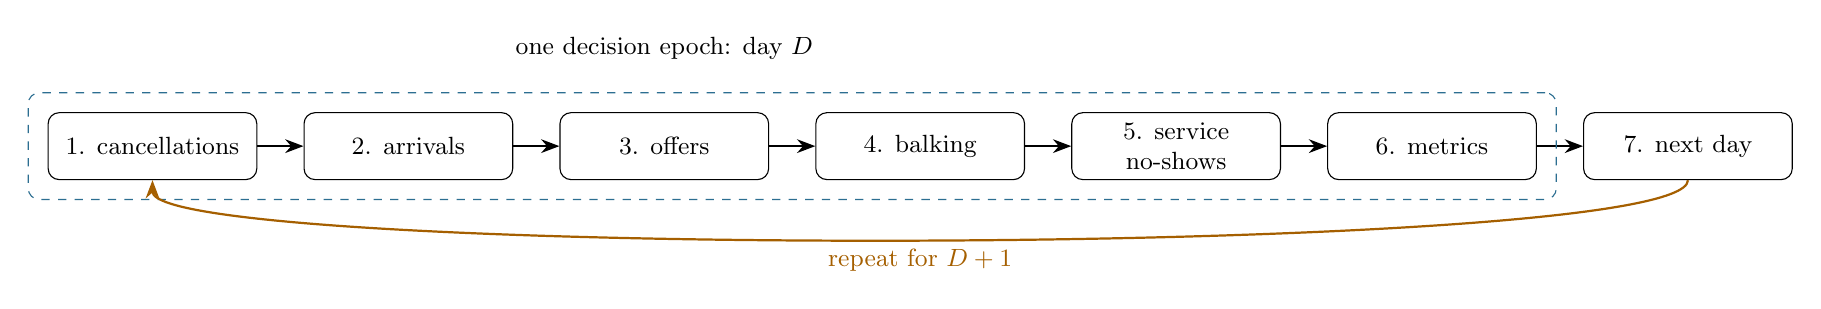
\begin{tikzpicture}[
    >=Stealth,
    every node/.style={font=\small},
    eventstep/.style={draw, rounded corners, align=center, minimum width=2.65cm, minimum height=0.85cm},
    band/.style={draw=FrameBlue, rounded corners, dashed, inner sep=7pt}
]
\node[eventstep] (c) at (0,0) {1. cancellations};
\node[eventstep] (a) at (3.25,0) {2. arrivals};
\node[eventstep] (o) at (6.50,0) {3. offers};
\node[eventstep] (b) at (9.75,0) {4. balking};
\node[eventstep] (s) at (13.00,0) {5. service\\no-shows};
\node[eventstep] (m) at (16.25,0) {6. metrics};
\node[eventstep] (n) at (19.50,0) {7. next day};

\draw[->, thick] (c) -- (a);
\draw[->, thick] (a) -- (o);
\draw[->, thick] (o) -- (b);
\draw[->, thick] (b) -- (s);
\draw[->, thick] (s) -- (m);
\draw[->, thick] (m) -- (n);
\node[band, fit=(c)(a)(o)(b)(s)(m)] {};
\node[above=0.55cm of o] {one decision epoch: day \(D\)};
\draw[->, thick, FrameGold] (n.south) .. controls +(0,-1.0) and +(0,-1.0) .. node[below] {repeat for \(D+1\)} (c.south);
\end{tikzpicture}
}
\end{center}

\begin{keybox}[title={Future-Only Cancellations and Offers}]
New arrivals on day \(D\) cannot book day \(D\). The cancellation step also applies only to future
appointments \(r=1,\dots,H-1\). Same-day occupancy is therefore resolved only through today's
no-show/service step, not through same-day cancellations or new offers.
\end{keybox}

\subsection{Calendar and Booking Logic}

\subsubsection{Day-Level Calendar Picture}

The old note used an \(H\times S\) slot calendar to show exactly where patients sat. The day-level
model uses the same rolling calendar concept, but it displays counts by class and residual day.

\begin{examplebox}[title={Visualizing the Day-Level State \(X^D\)}]
Suppose \(S=25\), \(H=4\), and after the cancellation step on day \(D\) the class-count state is:

\begin{center}
\renewcommand{\arraystretch}{1.45}
\setlength{\extrarowheight}{2pt}
\setlength{\tabcolsep}{7pt}
\resizebox{0.96\linewidth}{!}{
\begin{tabular}{|>{\raggedright\arraybackslash}m{2.8cm}|>{\centering\arraybackslash}m{2.0cm}|>{\centering\arraybackslash}m{2.0cm}|>{\centering\arraybackslash}m{2.0cm}|>{\centering\arraybackslash}m{2.0cm}|}
\hline
\rowcolor{gray!15}
\textbf{Count} & \shortstack{\textbf{day \(D\)}\\\(r=0\)} & \shortstack{\textbf{day \(D+1\)}\\\(r=1\)} & \shortstack{\textbf{day \(D+2\)}\\\(r=2\)} & \shortstack{\textbf{day \(D+3\)}\\\(r=3\)} \\
\hline
\cellcolor{gray!10}\(X_{1,r}^{D}\) & \cellcolor{blue!12}\calendarentry{9} & \cellcolor{blue!12}\calendarentry{12} & \cellcolor{blue!12}\calendarentry{8} & \cellcolor{blue!12}\calendarentry{5} \\
\hline
\cellcolor{gray!10}\(X_{2,r}^{D}\) & \cellcolor{orange!18}\calendarentry{11} & \cellcolor{orange!18}\calendarentry{13} & \cellcolor{orange!18}\calendarentry{10} & \cellcolor{orange!18}\calendarentry{7} \\
\hline
\cellcolor{gray!10}\(N_r^D\) & \calendarentry{20} & \cellcolor{red!12}\calendarentry{25} & \calendarentry{18} & \calendarentry{12} \\
\hline
\cellcolor{gray!10}\(S-N_r^D\) & \cellcolor{green!12}\calendarentry{5} & \cellcolor{red!12}\calendarentry{0} & \cellcolor{green!12}\calendarentry{7} & \cellcolor{green!12}\calendarentry{13} \\
\hline
\end{tabular}
}
\end{center}

The current day \(r=0\) has five open slots, but they are not bookable by new arrivals. Tomorrow
\((r=1)\) is full. The first eligible future day with capacity is \(r=2\), so the first offer under
FCFS is day \(D+2\), with \(\tau=2\).
\end{examplebox}

\subsubsection{FCFS Booking Rule}

For a new arrival on day \(D\), the baseline policy searches
\[
r=1,2,\dots,H-1
\]
and offers the first residual day satisfying
\[
N_r^D<S.
\]

If no such day exists, the patient receives no offer. If the patient accepts, the simulator
increments \(X_{i,r}^{D}\) and stores the patient's original delay as \(\tau=r\). If the patient
balks, \(X_{i,r}^{D}\) is not changed and the capacity remains available to later arrivals.

\subsection{Worked Day-Level Example}

This example is the day-level counterpart of the previous note's FCFS appointment-book example.
It shows the state, the patient audit record, the booking decision, the no-show/service step, and
the next-day rollover.

\begin{examplebox}[title={Worked Example: One Full Day \(D\)}]
Take \(S=25\), \(H=4\), and the post-cancellation state from the previous table:
\[
N_0^D=20,\qquad N_1^D=25,\qquad N_2^D=18,\qquad N_3^D=12.
\]
Assume that the cancellation step has already removed one future appointment, so the daily cancellation
counter is \(1\).

Daily arrivals are drawn once per class:
\[
M_1^D=14,\qquad M_2^D=10.
\]
The simulator randomizes the within-day order. In this realized day, the resulting offers can be
summarized by class mix and outcome.

The booking outcomes are:
\begin{center}
\small
\begin{tabular}{L{0.18\textwidth} L{0.20\textwidth} L{0.18\textwidth} L{0.30\textwidth}}
\toprule
\textbf{Group} & \textbf{Class mix} & \textbf{FCFS offer} & \textbf{Result} \\
\midrule
first cohort & \(4\) class 1, \(3\) class 2 & \(r=2,\ \tau=2\) & all \(7\) accept; day \(D+2\) becomes full \\
\addlinespace
second cohort & \(2\) class 2 & \(r=2,\ \tau=2\) & both balk; the remaining future capacity stays available \\
\addlinespace
third cohort & \(9\) class 1, \(4\) class 2 & \(r=3,\ \tau=3\) & all \(13\) accept; day \(D+3\) becomes full \\
\addlinespace
final cohort & \(1\) class 1, \(1\) class 2 & no future capacity & both receive no offer \\
\bottomrule
\end{tabular}
\normalsize
\end{center}

After offers and balking, the aggregate future counts are:
\[
N_0^D=20,\qquad N_1^D=25,\qquad N_2^D=25,\qquad N_3^D=25.
\]
The accepted patients are stored in the audit layer with their original delays: \(7\) bookings with
\(\tau=2\) and \(13\) bookings with \(\tau=3\). The balked and no-offer arrivals create no
appointment record.

Now the simulator resolves today's \(r=0\) appointments. Suppose \(17\) scheduled patients attend
and \(3\) no-show. Since \(S=25\) and only \(20\) patients were scheduled for today, the daily service
outcome is:
\[
\mathrm{served}=17,\qquad
\mathrm{no\_shows}=3,\qquad
\mathrm{empty\_slots}=5.
\]

Then the calendar advances. The full day \(D+1\) becomes the new current day, residual delays
decrease by one, and a new empty day \(D+4\) is appended:
\[
\left(N_0^{D+1},N_1^{D+1},N_2^{D+1},N_3^{D+1}\right)
=
(25,25,25,0).
\]
\end{examplebox}

\begin{examplebox}[title={Same Example as a Daily Progression Audit}]
The implementation exposes the same sequence through \texttt{daily\_progression}. A stylized row
for each step of the example is:

\begin{center}
\small
\resizebox{\linewidth}{!}{
\begin{tabular}{L{0.18\textwidth}rrrrrrrrL{0.28\textwidth}}
\toprule
\textbf{Step} & \textbf{Arr} & \textbf{Offer} & \textbf{Book} & \textbf{Balk} & \textbf{Canc} & \textbf{Served} & \textbf{NS} & \textbf{Empty} & \textbf{Interpretation} \\
\midrule
cancellations & 0 & 0 & 0 & 0 & 1 & 0 & 0 & 0 & one future appointment removed before arrivals \\
\addlinespace
arrivals & 24 & 0 & 0 & 0 & 1 & 0 & 0 & 0 & daily Poisson counts have been drawn \\
\addlinespace
offers and balking & 24 & 22 & 20 & 2 & 1 & 0 & 0 & 0 & future days \(D+2\) and \(D+3\) absorb \(20\) bookings; two arrivals balk and two get no offer \\
\addlinespace
no-shows/service & 24 & 22 & 20 & 2 & 1 & 17 & 3 & 5 & today's scheduled patients are resolved \\
\addlinespace
metrics & 24 & 22 & 20 & 2 & 1 & 17 & 3 & 5 & daily counters are ready for summaries \\
\addlinespace
advance & 24 & 22 & 20 & 2 & 1 & 17 & 3 & 5 & old \(r=1\) becomes the new \(r=0\) \\
\bottomrule
\end{tabular}
}
\normalsize
\end{center}

This table is not a second model. It is an audit view of the model order. It exists so a reader can
verify that the simulator is progressing exactly one day at a time.
\end{examplebox}

\section{Outputs and Code Mapping}

\subsection{Performance Measures}

For patients arriving during the measured window, the simulator reports:
\begin{center}
\small
\begin{tabular}{L{0.28\textwidth} L{0.62\textwidth}}
\toprule
\textbf{Metric} & \textbf{Definition} \\
\midrule
Arrivals & number of appointment requests \\
\addlinespace
Booked & number of requests that accept an offer \\
\addlinespace
Balked & number of requests that receive an offer and decline it \\
\addlinespace
No offer & number of requests for which no future capacity is available \\
\addlinespace
Canceled & number of booked patients who cancel before service resolution \\
\addlinespace
No-shows & number of booked patients who remain scheduled but do not attend \\
\addlinespace
Served & number of booked patients who attend \\
\addlinespace
Mean booked delay & average original offered delay \(\tau\) among booked patients \\
\bottomrule
\end{tabular}
\normalsize
\end{center}

The main access and service ratios are:
\[
\frac{\mathrm{Booked}}{\mathrm{Arrivals}},
\qquad
\frac{\mathrm{Served}}{\mathrm{Booked}},
\qquad
\frac{\mathrm{Booked\ within\ target}}{\mathrm{Arrivals}}.
\]

For measured service days, daily capacity is still \(S\). Slot utilization is therefore:
\[
\rho^{\mathrm{booked}}
=
\frac{\mathrm{booked\ slots}}{S\times\mathrm{measured\ days}},
\qquad
\rho^{\mathrm{attended}}
=
\frac{\mathrm{served\ slots}}{S\times\mathrm{measured\ days}}.
\]

\subsection{Implementation Mapping}

The code follows this day-level formulation:
\begin{itemize}[nosep]
    \item \texttt{arrival\_rate} is \(\lambda_i\), the expected class-\(i\) arrivals per day.
    \item \texttt{cancel\_probability} as a scalar is the direct daily cancellation probability \(\phi_i\) for appointments still scheduled in the future.
    \item \texttt{tau\_offered} and \texttt{tau\_booked} are original offered delays in days.
    \item \texttt{arrival\_slot} is retained as a legacy log column and is empty under the day-level process.
    \item \texttt{state\_log} records \(X_{i,r}^{D}\) for every configured class and residual day.
    \item \texttt{daily\_progression} records the seven daily model steps for each measured day.
    \item \texttt{slots\_per\_day} is daily capacity \(S\), and remains the denominator for slot utilization.
\end{itemize}

\begin{reviewbox}[title={Review Against the Intended New Model}]
\begin{itemize}[nosep]
    \item The model state is day/class count state \(X_{i,r}^{D}\), not slot state \(Y_t(r,m)\).
    \item The arrival rate \(\lambda_i\) is daily, so \(M_i^D\sim\mathrm{Poisson}(\lambda_i)\).
    \item Same-day offers are disabled; bookable residual days are \(r=1,\dots,H-1\).
    \item Scalar \(\phi_i\) is a daily cancellation probability applied once per day to future appointments \(r=1,\dots,H-1\).
    \item A booked patient's original \(\tau\) is retained for balking, no-show, advanced cancellation rules, and delay metrics.
    \item The event order is cancellations, arrivals, offers, balking, no-shows/service, metrics, and calendar advance.
\end{itemize}
\end{reviewbox}

\section{Literature and Scope}

\subsection{Relation to the Literature}

Green and Savin (2008), Liu and Ziya (2014), and Liu (2015) use stylized queue, backlog, or window
states to study delay-sensitive attendance and appointment access. The day-level simulator is a
calendar version of the same mechanism. The state \(X_{i,r}^{D}\) records the future schedule by
class and residual day; the offered delay \(\tau\) is the calendar analog of the congestion seen by
the patient at booking.

\subsubsection{Common Mechanism}

The analytical papers usually compress the appointment book into one congestion variable, such as
queue length, backlog, or the number of appointments already ahead of a new patient. This note keeps
the appointment book explicit but day-level:
\[
X^D=\left(X_{i,r}^{D}:i\in\mathcal I,\ r=0,\dots,H-1\right).
\]
Under FCFS, this state implies the offered delay
\[
\tau
=
\min\{r\in\{1,\dots,H-1\}:N_r^D<S\},
\]
when such an \(r\) exists. Thus \(\tau\) is the bridge between the calendar model and the queueing
literature. A larger backlog pushes the first feasible \(r\) farther into the future, and that
larger \(\tau\) then enters \(b_i(\tau)\) and the baseline step no-show rule \(\xi_i(\tau)\). In
later experiments, the smoother advanced rule \(\tilde{\xi}_i(\tau)\) can be used instead. In the
baseline, cancellation is the scalar daily probability \(\phi_i\). Later experiments can replace it
with the advanced rule \(\tilde{\phi}_i(\tau,r)\).

\begin{keybox}[title={Why the Day-Level Model Still Matches the Literature}]
The literature does not require a slot index to create delay feedback. It requires a congestion
state that determines the delay seen at booking. In v2, \(X^D\) is that state, and FCFS converts it
into the offered delay \(\tau\).
\end{keybox}

\subsubsection{Green and Savin (2008)}

Green and Savin study an appointment queue in which no-show behavior worsens with the backlog seen
when the appointment is made. Their no-show curve is an exponential-saturation function of a
congestion measure. The v2 baseline deliberately simplifies that behavior to a step function
\(\xi_i(\tau)\) so the daily progression stays easy to read, but it keeps the Green-Savin shape as
the advanced option
\[
\tilde{\xi}_i(\tau)
=
\gamma_{i,\max}
-
(\gamma_{i,\max}-\gamma_{i,0})e^{-\tau/s_i}.
\]

The mapping is:
\begin{itemize}[nosep]
    \item their backlog variable maps to the FCFS delay implied by \(X^D\);
    \item their no-show mechanism maps directly to \(\tilde{\xi}_i(\tau)\), while the baseline \(\xi_i(\tau)\) is a step approximation used for the first FCFS experiments;
    \item their homogeneous queue is extended here to multiple classes through \(i\);
    \item v2 also adds explicit balking and pre-appointment cancellation.
\end{itemize}

The simplification in v2 is that time advances by day rather than by individual service slot. This
is acceptable for the first simulator because the central feedback loop depends on appointment
delay in days, not on the exact within-day slot where the appointment sits.

\subsubsection{Liu and Ziya (2014)}

Liu and Ziya analyze panel size and overbooking decisions under patient no-shows. Their state is
more stylized than a rolling calendar, but the core tradeoff is the same: more demand can increase
utilization, while longer waits can reduce realized attendance.

The v2 simulator intentionally does not optimize panel size or overbooking yet. It fixes daily
capacity \(S\), uses FCFS, and observes how access, booking, cancellation, no-show, and service
metrics respond to demand and behavior. This makes the simulator a diagnostic baseline before any
future optimization layer is added.

The mapping is:
\begin{itemize}[nosep]
    \item their panel size / demand pressure maps to total daily arrival rate \(\lambda\);
    \item their show-up probability maps to \(1-\xi_i(\tau)\) in the baseline and \(1-\tilde{\xi}_i(\tau)\) in the more detailed variant;
    \item their capacity decision maps here to fixed daily capacity \(S\);
    \item their overbooking decision is not active in the v2 FCFS baseline.
\end{itemize}

\subsubsection{Liu (2015)}

Liu studies the optimal appointment scheduling window under delay-dependent no-shows. The model's
window size limits how far into the future appointments may be scheduled. In v2, the rolling
horizon \(H\) plays the same operational role:
\[
r\in\{0,1,\dots,H-1\}.
\]

Because same-day offers are disabled in the current baseline, the bookable window is
\[
r\in\{1,\dots,H-1\}.
\]
If every future residual day is full, the arriving patient receives no offer. This is the explicit
calendar equivalent of a finite scheduling window rejecting or deferring demand when the window is
full.

The mapping is:
\begin{itemize}[nosep]
    \item Liu's appointment window \(K\) maps to the simulator horizon \(H\);
    \item delay-sensitive attendance maps to \(\xi_i(\tau)\) in the baseline and to \(\tilde{\xi}_i(\tau)\) in the more detailed variant;
    \item the no-offer event appears when the FCFS search over \(r=1,\dots,H-1\) finds no capacity;
    \item optimizing \(H\) is a later experiment, not part of the current FCFS-only baseline.
\end{itemize}

\subsubsection{Why Only FCFS Here}

The old codebase already supports alternative slot-selection policies, but this note deliberately
keeps the analysis focused on FCFS. That is the cleanest first experiment because it isolates the
baseline delay-feedback mechanism:
\[
X^D
\rightarrow
\tau_{\mathrm{FCFS}}
\rightarrow
b_i(\tau),\ \phi_i,\ \xi_i(\tau)
\rightarrow
\text{daily outcomes}.
\]

Future policies can be introduced later as changes to the arrival, admission, or offer step. They
should be compared against this FCFS baseline only after the day-level mechanics and metrics are
stable.

\begin{center}
\small
\begin{tabular}{L{0.18\textwidth} L{0.22\textwidth} L{0.22\textwidth} L{0.24\textwidth}}
\toprule
\textbf{Model / paper} & \textbf{State abstraction} & \textbf{Delay variable} & \textbf{Difference from this simulator} \\
\midrule
Green and Savin (2008) & queue length / backlog & backlog seen when appointment is made & analytical single-class queue; no explicit calendar \\
\addlinespace
Liu and Ziya (2014) & queue length in appointment model & congestion at booking time & optimizes panel size and overbooking \\
\addlinespace
Liu (2015) & finite appointment window & delay implied by the scheduling window & optimizes the window size \(K\) \\
\addlinespace
This simulator v2 & rolling day-count calendar \(X_{i,r}^{D}\) & original offered delay \(\tau\) & two classes, cancellations, balking, and explicit daily progression \\
\bottomrule
\end{tabular}
\normalsize
\end{center}

\section{References}

\begin{itemize}[itemsep=0.25em]
    \item Green, L. V., and S. Savin. 2008. Reducing delays for medical appointments: A queueing approach. \emph{Operations Research} 56(6):1526--1538.
    \item Liu, N. 2015. Optimal choice for appointment scheduling window under patient no-show behavior. \emph{Production and Operations Management} 25(1):128--142.
    \item Liu, N., and S. Ziya. 2014. Panel size and overbooking decisions for appointment-based services under patient no-shows. \emph{Production and Operations Management} 23(12):2209--2223.
\end{itemize}

\end{document}
